% !Mode:: "TeX:UTF-8"

\section{已完成的研究工作}
\subsection{同步偏差对混合载波通信系统的影响}

混合载波通信系统发射信号会同时包含单载波分量和多载波分量。也就是说变换域通信系统的信号特征同时继承了单载波通信系统和多载波通信系统的信号特点,然而也同样因此不仅继承了两种通信系统的优点,也保留了缺点。我们知道,单载波系统由于其在时域中进行符号判决,因而对定时偏差非常敏感,而多载波系统由于传输性能是仪子载波间的正交性为基础的,很小的频率偏差就会破坏正交性,从而极大影响系统性能,因此对于混合载波通信系统而言,精准的定时同步和频率偏差矫正非常重要。

在实际通信系统中,引起同步误差最主要的原因是收发双方晶振时钟不一致,从而导致的在接收端的采样时刻的误差和收发双方的载波频率不同步, 根据前面已经分析了混合载波的通信系统模型,图~\ref{jiaquanshixianguocheng}~给出存在同步偏差的信道模型:
\begin{figure}[htbp]
\centering
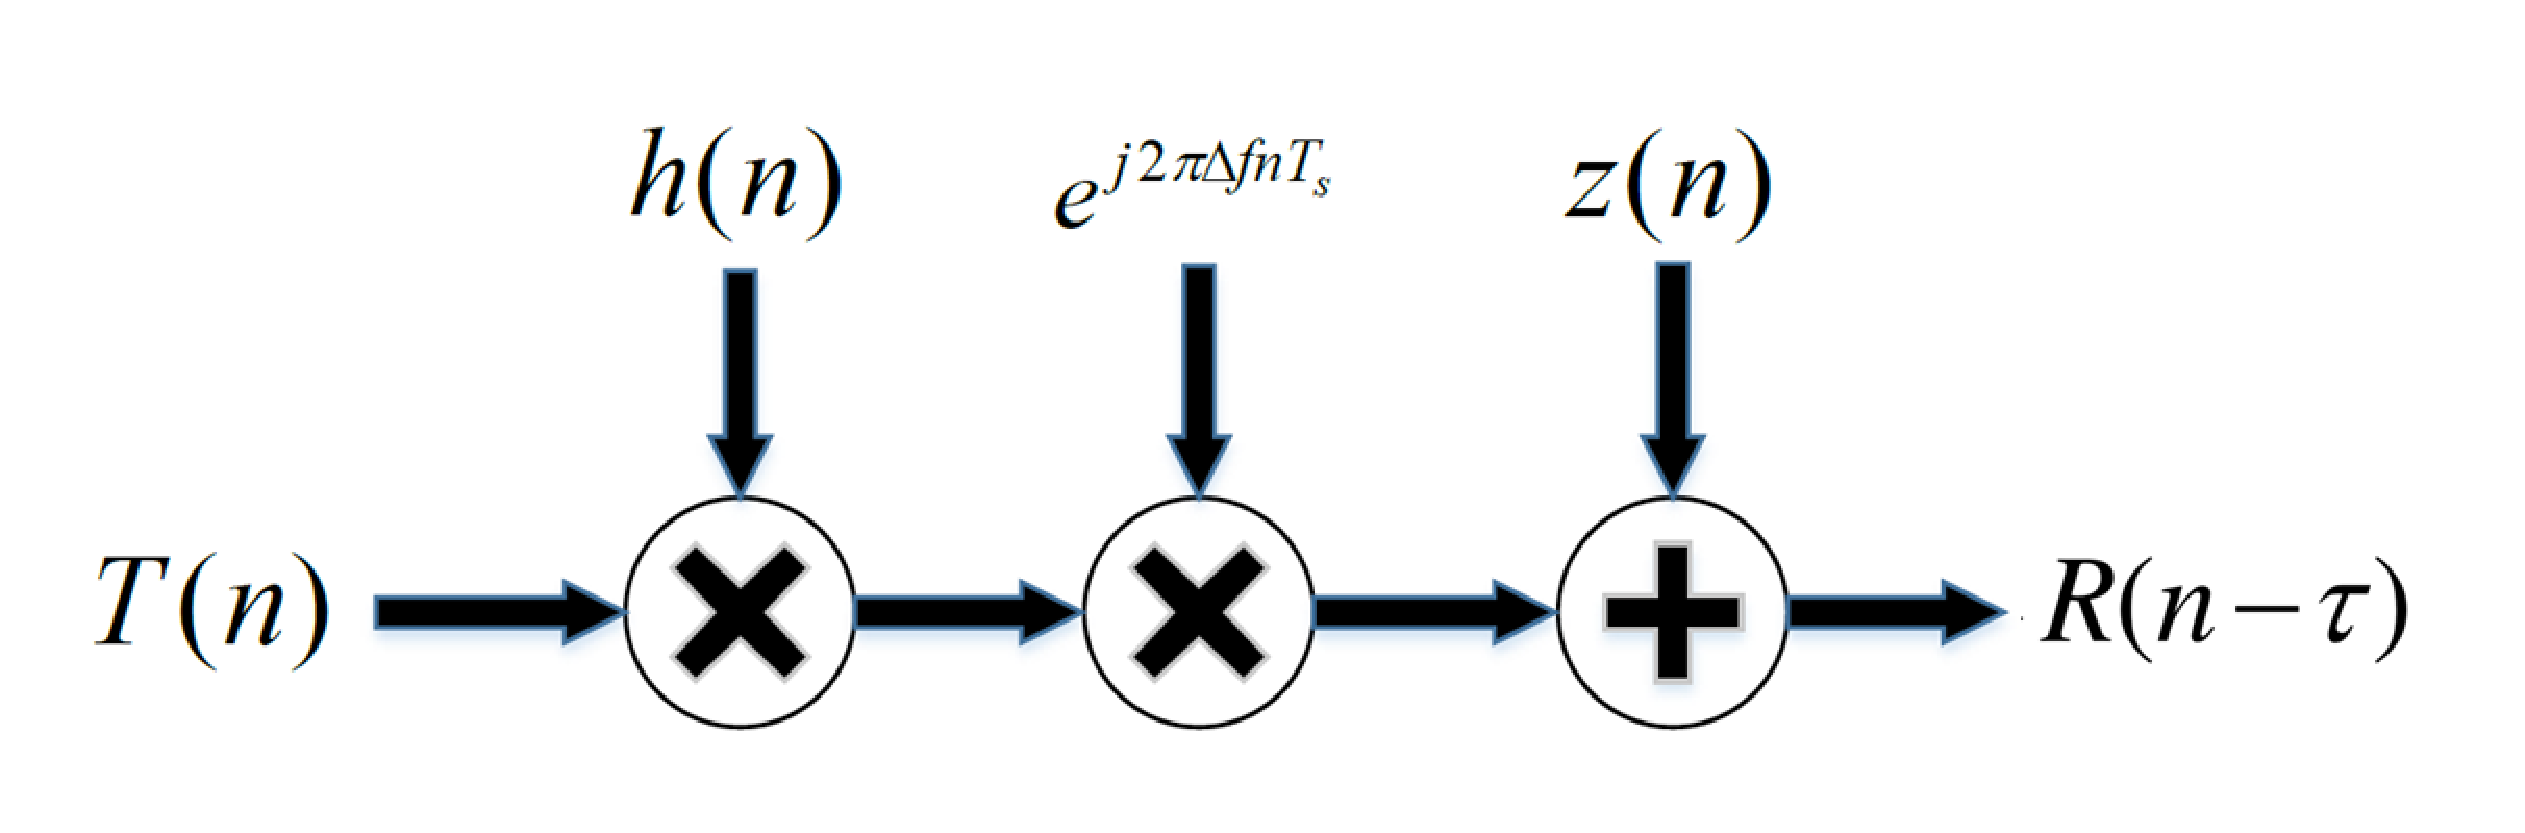
\includegraphics[width = 0.6\textwidth]{figure4_1.eps}
\caption{信道模型}\vspace{-1em}\label{xindaomoxing}
\end{figure}
其中~$T(n)$~为混合载波通信系统发射端发送到信道中的时域信号,即基带调制后的信号~$X(n)$~进行~$\alpha$~阶~4-WFRFT~变换的结果,$h(n)$~为信道的冲激相应,$R(n)$~为发射信号~$T(n)$~经过信道并且在接收端下变频后接收到的信号。为了后续理论分析与讨论的简便,这里假设信道是平缓的即~$h(n)=1$,信号仅受到频偏与加性高斯白噪声~$z(n)$~的影响,并在接受端存在一定时延。这里简化系统发射接收时上下变频的过程,将发射端与接收端由于晶振偏差产生的本地载波频率偏差引入到信道中,其中~$\Delta f$~表示发射与接收端本地载波频差,$T_s$~表示发送端基带数据采样间隔。

根据前面的~WFRFT~理论,设变换前基带信号为~$X(n)$~,
%则发射信号如公式~(\ref{fashexinhao})~所示
%\begin{equation}\label{fashexinhao}
%\begin{split}
%T(n) = w_0^\alpha X(n) + w_1^\alpha  \cdot \frac{1}{{\sqrt N }}\sum\limits_{k = 0}^{N - 1} {X(k){e^{ - j\frac{{2\pi }}{N}kn}}} \\
%  + w_2^\alpha X( - n) + w_3^\alpha  \cdot \frac{1}{{\sqrt N }}\sum\limits_{k = 0}^{N - 1} {X(k){e^{j\frac{{2\pi }}{N}kn}}}
%\end{split}
%\end{equation}
这里为了讨论方便,将分别推导采样时间偏差和频率偏差对混合载波通信系统影响。首先讨论当仅存在定时偏差的情况,混合载波定时同步的示意图如下:
\begin{figure}[htbp]
\centering
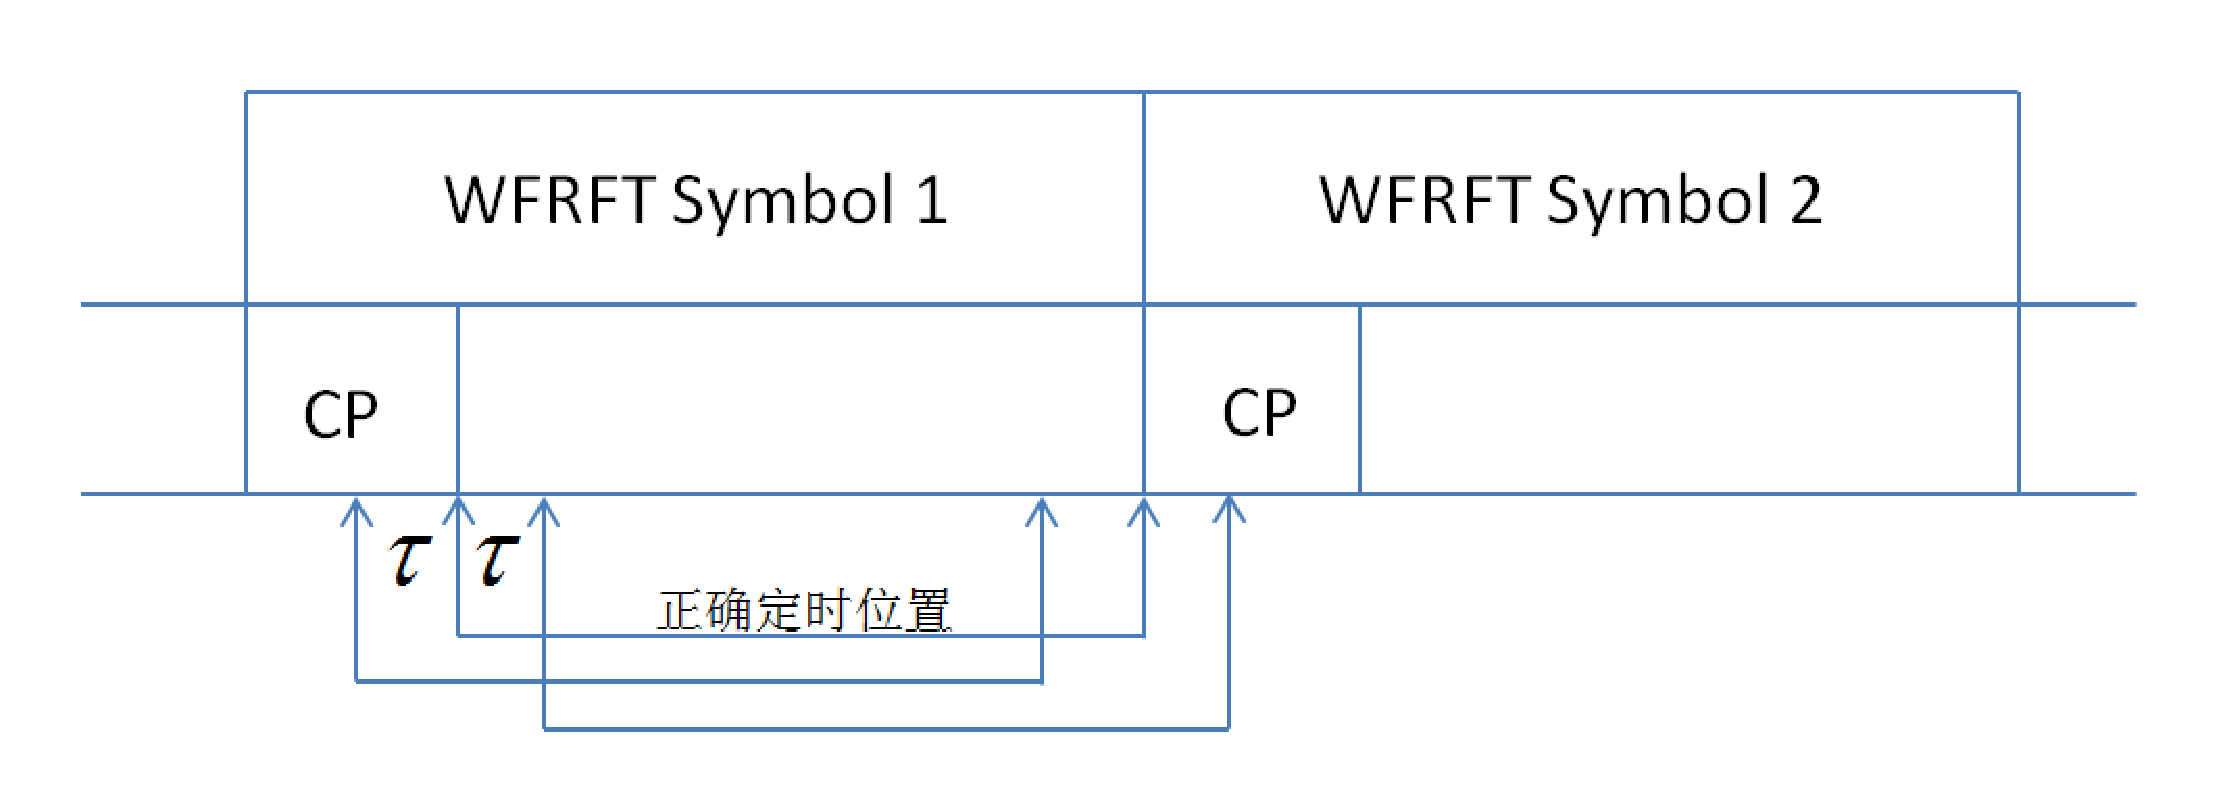
\includegraphics[width = 0.8\textwidth]{figure4_2.eps}
\caption{定时同步示意图}\vspace{-1em}\label{dingshitongbuweizhi}
\end{figure}

接收端的基带信号表现形式如下:
\begin{equation}
R(n-\tau) = T(n-\tau) + z(n-\tau)
\end{equation}

当接收端时间同步不精确,定时同步的起点位于循环前缀内部时,
\begin{align}\label{}
\tilde X_i(n) &= {\mathcal{F}^\alpha }\left ( R_i\left ( n-\tau \right ) \right ) \nonumber \\
&= w_0^{- \alpha }R_i(n-\tau) + w_1^{- \alpha }{{\mathcal{F}^1}\left ( R_i\left ( n-\tau \right ) \right )}
+ w_2^{- \alpha }{{\mathcal{F}^2}\left ( R_i\left ( n-\tau \right ) \right )}
+ w_3^{- \ }{{\mathcal{F}^3}\left ( R_i\left ( n-\tau \right ) \right )} \nonumber \\
&= \underbrace {w_0^{- \alpha }R_i(n-\tau) + w_2^{- \alpha }R_i(\tau -n)}_{ISI} + w_1^{- \alpha }{{\mathcal{F}}\left ( R_i\left ( n \right ) \right )} {e^{-j2\pi \frac{{\varepsilon n}}{N}}} + w_3^{- \alpha }{{\mathcal{F}}\left ( R_i\left ( -n \right ) \right )} {e^{-j2\pi \frac{{\varepsilon n}}{N}}}
\end{align}

其中~$R_i(n)$~代表接受到的第i个WFRFT符号的第~$n$~个采样点,从式中可以看出,由于单载波分量的存在,定时同步误差将引入符号间干扰(ISI),而第二与第四分量虽然会产生一个相位因子,但并未产生干扰。而若当定时同步起点位于循环前缀外时,此时这一符号的采样信息会包含下一符号的信息,不仅引入了符号间干扰,同时也会在多载波分量间引入载波间干扰~ICI,这种情况下将严重影响通信性能,应是极力避免的,在此便不详细推导了。
\begin{figure}[htbp]
\centering
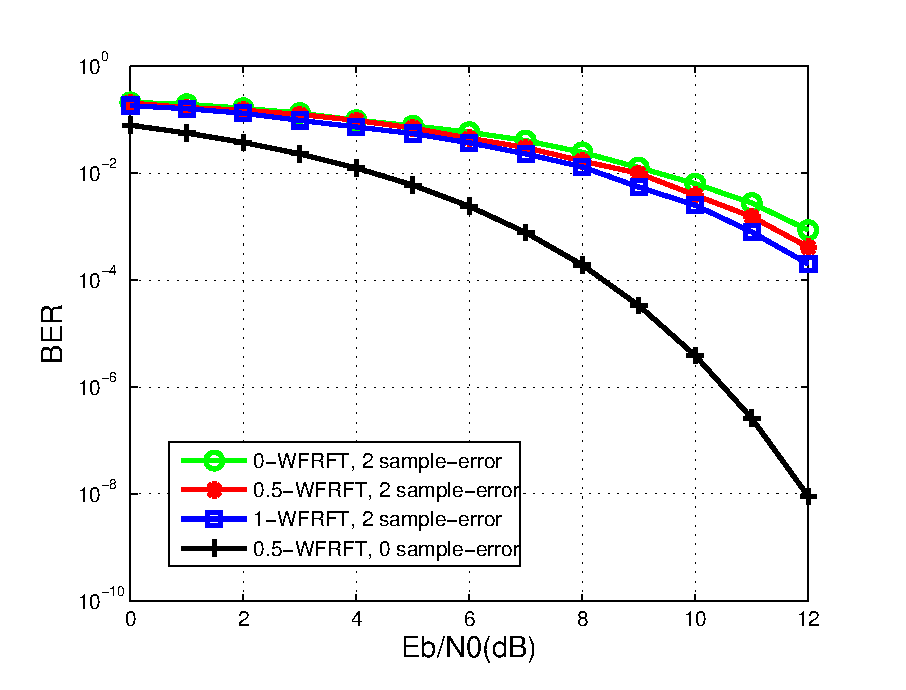
\includegraphics[width = 0.8\textwidth]{plot_ber_at_time_error.eps}
\caption{不同调制阶数下HC系统在2个定时误差下误码性能比较}\vspace{-1em}\label{plot_ber_at_time_error}
\end{figure}

图~\ref{plot_ber_at_time_error}~给出了~AWGN~信道下混合载波通信系统当在非最佳采样点下误码性能的比较,仿真参数选择一个~WFRFT~符号载波数为~2048,数据符号所占载波数为~1200,采用~16~倍上采样,收发双方均采用升余弦滚降滤波器进行滤波,在接受端存在~2~个采样点的误差进行解调下,当调制阶数~1~时,此时混合载波通信系统只包含多载波通信过程,此时系统抗定时误差性能最好。当调制阶数~0~时,混合载波通信系统只包含单载波成分,其性能受定时误差影响较大大。当调制阶数介于~0~到~1~之间时,此时混合载波通信系统同时包含有单载波成分和多载波成分,且阶数越小,包含的单载波成分也越多,此时受定时采样误差影响也越大。图中黑线为无采样点偏差下的混合载波通信系统误码率性能,从图中也可以看出,虽然仅仅有~2~个采样点误差,但与最佳采样点的系统性能相差巨大,故定时同步对系统性能的保证十分关键。

另一方面,当混合载波通信系统中存在频偏影响时,发射信号受到频偏的影响在接收端的基带信号表示形式如为~$R(n) = T(n){e^{j2\pi \Delta f(n){T_s}}} + z(n)$~。接收端的解调过程需对接收信号进行~$-\alpha$~阶~4-WFRFT~变换以恢复原始信号~$X(n)$~,将接收信号代入解调公式可以得出解调结果数学表达式如公式~(\ref{jietiaojieguo})~所示:
\begin{eqnarray}\label{jietiaojieguo}
%\begin{array}{l
\tilde X(n) &=& (w_0^{ - \alpha }w_0^\alpha  + w_2^{ - \alpha }w_2^\alpha )X(n){e^{j2\pi \frac{{\varepsilon n}}{N}}} \nonumber \\
&+& {\rm{ }}w_1^{ - \alpha }w_3^\alpha \frac{1}{N}\sum\limits_{k = 0}^{N - 1} {\sum\limits_{m = 0}^{N - 1} {X(m){e^{j2\pi \frac{{mk}}{N}}}{e^{j2\pi \frac{{\varepsilon k}}{N}}}{e^{ - j2\pi \frac{{kn}}{N}}}} } \nonumber \\
&+& {\rm{ }}w_3^{ - \alpha }w_1^\alpha \frac{1}{N}\sum\limits_{k = 0}^{N - 1} {\sum\limits_{m = 0}^{N - 1} {X(m){e^{ - j2\pi \frac{{mk}}{N}}}{e^{j2\pi \frac{{\varepsilon k}}{N}}}{e^{j2\pi \frac{{kn}}{N}}}} } \nonumber \\
&+& {\rm{ (}}w_0^{ - \alpha }w_1^\alpha  + w_1^{ - \alpha }w_0^\alpha  + w_2^{ - \alpha }w_3^\alpha  + w_3^{ - \alpha }w_2^\alpha )\frac{1}{N}\sum\limits_{k = 0}^{N - 1} {\sum\limits_{m = 0}^{N - 1} {X(m){e^{ - j2\pi \frac{{mk}}{N}}}{e^{j2\pi \frac{{\varepsilon k}}{N}}}{e^{ - j2\pi \frac{{kn}}{N}}}} } \nonumber \\
&+& {\rm{ (}}w_3^{ - \alpha }w_1^\alpha  + w_1^{ - \alpha }w_3^\alpha  + w_1^{ - \alpha }w_2^\alpha  + w_2^{ - \alpha }w_1^\alpha )\frac{1}{N}\sum\limits_{k = 0}^{N - 1} {\sum\limits_{m = 0}^{N - 1} {X(m){e^{j2\pi \frac{{mk}}{N}}}{e^{j2\pi \frac{{\varepsilon k}}{N}}}{e^{j2\pi \frac{{kn}}{N}}}} } \nonumber \\
&+& Z(n)
%\end{array}
\end{eqnarray}
式中~$\varepsilon  = \Delta fN{T_s}$~表示归一化频偏,$N$~为~4-WFRFT~一个符号的变换点数。~$Z(n)$~表示高斯白噪声经过~$-\alpha$~阶~4-WFRFT~变换的结果仍为高斯白噪声。又由于加权系数~$w$~的定义,不难推导出
\begin{equation}
\left\{ \begin{array}{l}
{\rm{(}}w_0^{ - \alpha }w_1^\alpha  + w_1^{ - \alpha }w_0^\alpha  + w_2^{ - \alpha }w_3^\alpha  + w_3^{ - \alpha }w_2^\alpha ) = 0\\
{\rm{(}}w_3^{ - \alpha }w_1^\alpha  + w_1^{ - \alpha }w_3^\alpha  + w_1^{ - \alpha }w_2^\alpha  + w_2^{ - \alpha }w_1^\alpha ) = 0
\end{array} \right.
\end{equation}
再记
\begin{equation}
{\lambda _{m - n}} = w_1^{ - \alpha }w_3^\alpha \frac{1}{N}\sum\limits_{k = 0}^{N - 1} {{e^{j2\pi (m - n + \varepsilon )k/N}}}  + w_3^{ - \alpha }w_1^\alpha \frac{1}{N}\sum\limits_{k = 0}^{N - 1} {{e^{j2\pi (n - m + \varepsilon )k/N}}}
\end{equation}
为变换域~ICI~系数。对式~(\ref{jietiaojieguo})~进一步化简得到式~(\ref{huajianjieguo})~
\begin{align}\label{huajianjieguo}
\tilde X(n) &= (w_0^{ - \alpha }w_0^\alpha  + w_2^{ - \alpha }w_2^\alpha )X(n){e^{j2\pi \frac{{\varepsilon n}}{N}}} + \sum\limits_{m = 0}^{N - 1} {X(m){\lambda _{m - n}}}  + Z(n) \nonumber \\
&= \underbrace {(w_0^{ - \alpha }w_0^\alpha  + w_2^{ - \alpha }w_2^\alpha )X(n){e^{j2\pi \frac{{\varepsilon n}}{N}}} + X(n){\lambda _0}}_{C(n)} + \underbrace {\sum\limits_{m = 0,m \ne n}^{N - 1} {X(m){\lambda _{m - n}}} }_{ICI(n)} + Z(n)
\end{align}
其中~$C(n)$~表示系统有用信号,$ICI(n)$~表示频偏引起的载波间相互影响带来的干扰信号。

图~\ref{plot_ber_at_freq_error}~给出了~4-WFRFT~变换域通信系统在调制阶数~$\alpha$~时,归一化频偏~$\varepsilon$~分别为~0~,0.03~,0.05~,0.1~时的误码率性能比较。
\begin{figure}[htbp]
\centering
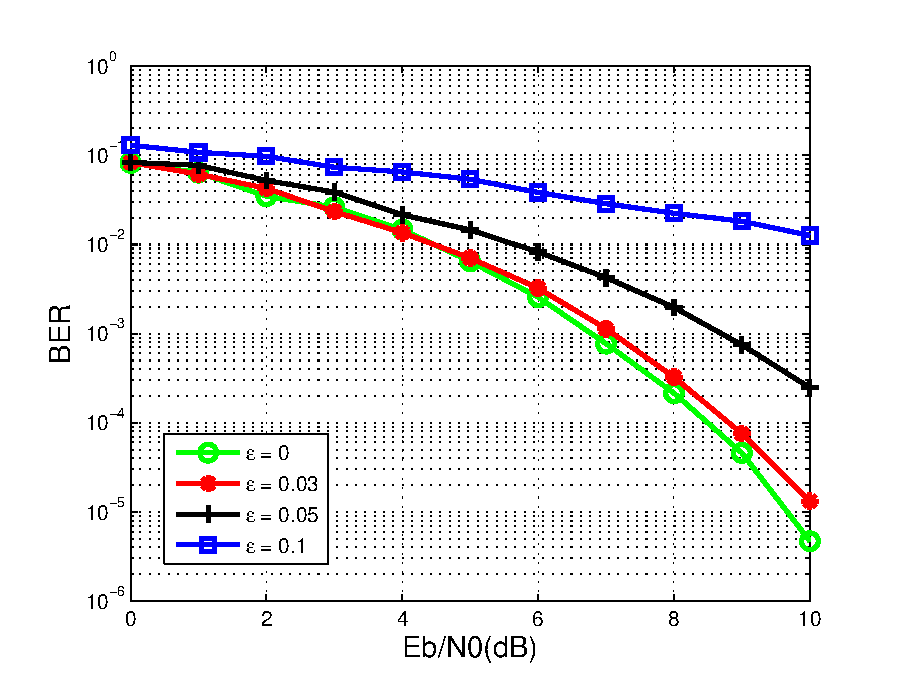
\includegraphics[width = 0.8\textwidth]{plot_ber_at_freq_error.eps}
\caption{有频偏下误比特率比较}\vspace{-1em}\label{plot_ber_at_freq_error}
\end{figure}
仿真数据采用~QPSK~调制。从图中可以看出,随着归一化频偏逐渐提高,变换域通信系统受到频偏的影响逐渐增大,性能逐渐降低。当归一化频偏达到~0.1~时系统性能已经严重下降。因此,在接收端频率同步就显得十分必要。


\subsection{基于循环前缀的同步算法}


我们知道,在~OFDM~技术中,为了消除码间干扰,对抗多径,传输信号使用了适当的循环前缀技术,只要循环前缀的长度大于无线信道中的最大时延扩展,这样一个符号的多径分量就不会对下一个符号产生干扰,也不会因为多径的影响破坏子载波间的正交性。在混合载波通信系统中仍将采用分组传输的思想,利用循环前缀技术来对抗多径。根据最大似然原理的基本思想,可以利用发送信号结构中的循环前缀与信号本身的相关性来实现信号同步。

目前现有的基于循环前缀的比较经典的同步算法是文献\cite{Jan1997ML}中提出的基于最大似然概率的同步算法,可将其应用在混合载波通信系统中。ML~算法对于定时和频偏的估计是以假设信道为加性高斯白噪声为前提的。这里给定~AWGN~信道下接收信号如下:
\begin{equation}
R(n) = T(n-\theta){e^{j2\pi \varepsilon k/N} } + z(n)
\end{equation}
~$\theta$~表示信号未确定的到达时间,$\varepsilon$~是归一化频偏。

ML~算法信号结构如图~\ref{ML_symbol_figure},
\begin{figure}[htbp]
\centering
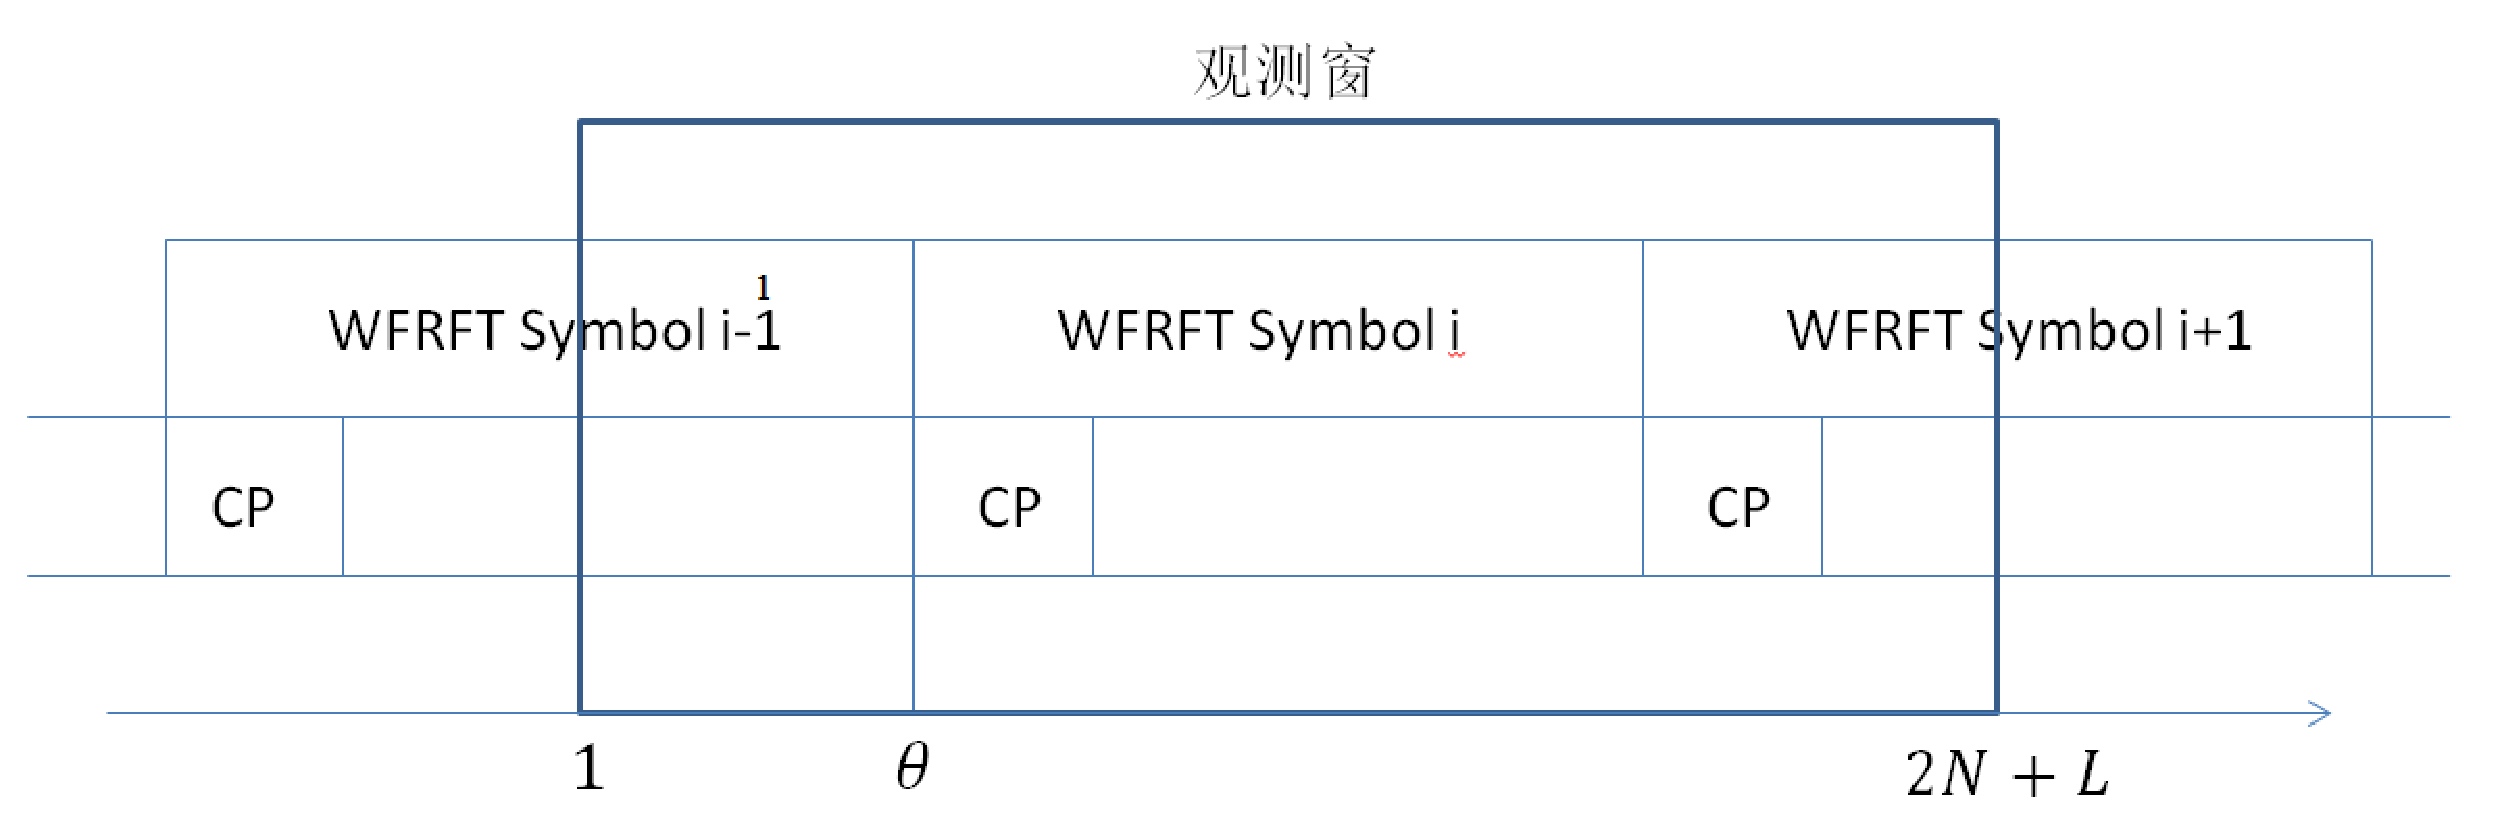
\includegraphics[width = 0.8\textwidth]{ML_symbol_figure.eps}
\caption{~ML~算法信号结构}\vspace{-1em}\label{ML_symbol_figure}
\end{figure}
假定一个~WFRFT~符号长度为~N,循环前缀长度为~L,我们将观测窗长度定为~$2N+L$,这样我们得到的采样点中包含一个完整的~WFRFT~符号(包含~$N+L$~采样点)。在这组采样点块中,符号的起始位置~$\theta$~对于接收端是未知的。观察窗口内接收信号的~$2N+L$~个采样值在给定同步参数定时误差~$\theta$~和频率偏移~$\varepsilon$~时的联合条件概率密度函数为:
\begin{equation}
\Lambda \left( {\theta ,\varepsilon } \right) = \log f\left( {r|\theta ,\varepsilon } \right)
\end{equation}
基于循环前缀同步的原理就是求使得~$\Lambda \left( {\theta ,\varepsilon } \right)$~最大时的定时误差和频率偏移。文献\cite{Jan1997ML}中对其进行化简推导得到
\begin{equation}
\Lambda \left( {\theta ,\varepsilon } \right) = \left| {\gamma \left( \theta  \right)} \right|\cos \left( {2\pi \varepsilon  + \angle \gamma \left( \theta  \right)} \right) - \rho \phi \left( \theta  \right)
\end{equation}
其中~$\angle$~为复数角度算子
\begin{equation}
\gamma \left( m \right) = \sum\limits_{k = m}^{m + L - 1} {r\left( k \right){r^*}\left( {k + N} \right)} ,
\end{equation}
\begin{equation}
\phi \left( m \right) = \frac{1}{2}\sum\limits_{k = m}^{m + L - 1} {{{\left| {r\left( k \right)} \right|}^2} + {{\left| {r\left( {k + N} \right)} \right|}^2}}
\end{equation}
\begin{equation}
\rho  = \left| {\frac{{E\left\{ {r\left( k \right){r^*}\left( {k + N} \right)} \right\}}}{{\sqrt {E\left\{ {{{\left| {r\left( k \right)} \right|}^2}} \right\}E\left\{ {{{\left| {r\left( {k + N} \right)} \right|}^2}} \right\}} }}} \right| = \frac{{\sigma _s^2}}{{\sigma _s^2 + \sigma _n^2}} = \frac{{SNR}}{{SNR + 1}}
\end{equation}

为了使最大似然函数能取得最大值,其中余弦项需为~1,似然函数变为
\begin{equation}
\Lambda \left( {\theta ,\varepsilon } \right) = \left| {\gamma \left( \theta  \right)} \right| - \rho \phi \left( \theta  \right)
\end{equation}
对~$\theta$~和~$\varepsilon$~的联合最大似然估计为
\begin{align}
&{\hat \theta _{ML}} = \arg \mathop {\max }\limits_\theta  \left\{ {\left| {\gamma \left( \theta  \right)} \right| - \rho \phi \left( \theta  \right)} \right\} \\
&{\hat \varepsilon _{ML}} =  - \frac{1}{{2\pi }}\angle \gamma \left( {{{\hat \theta }_{ML}}} \right)
\end{align}

图~\ref{ML_sim1}~给出~ML~算法的信号仿真,一个~WFRFT~符号长度选择~1024~点,循环前缀长度为~128~点,频率偏差为给定值~0.25,信噪比~$SNR=15dB$。图中上图表示最大似然函数随在不同采样起始时刻的最大模值,下图为在该采样时刻作为起始时刻所估计出来的归一化频率偏移值。
\begin{figure}[htbp]
\centering
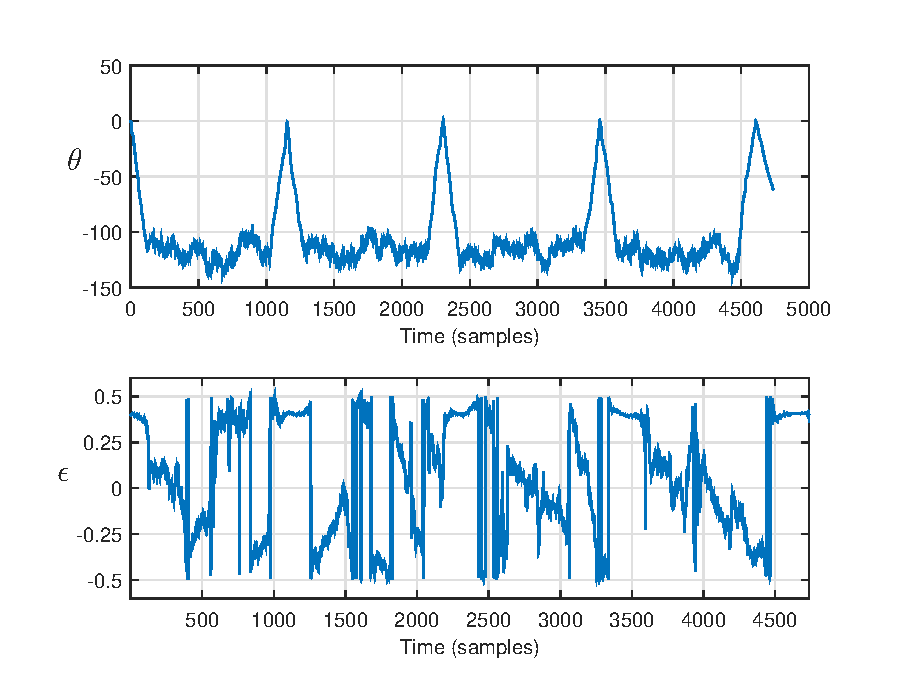
\includegraphics[width = 0.8\textwidth]{ML_sim1.eps}
\caption{~ML~算法信号仿真}\vspace{-1em}\label{ML_sim1}
\end{figure}
从图中可以看出,ML~算法的定时偏差估计曲线在正确的~CP~起始位置有着非常尖锐的峰值。仿真中存在~5~个~WFRFT~符号,所以有五个峰值,作为符号定时偏移的估计。其中横坐标为采样的点数,纵坐标为似然函数的值。在测度函数的最大值就是正确定时时刻。基于这一正确的符号定时点,又可以得出频偏的正确估
计值,如图。仿真时设定的频率偏移为~0.25。可以看到,在正确的定时估计位置,对应的频率偏移都在~0.25~左右。

下面通过仿真分析~ML~算法的性能,性能指标为定时偏移和频率偏差估计的均方误差。首先参数估计的均方误差随偏差值大小的关系如图~\ref{Performance_by_freqError}~。
\begin{figure}[htbp]
\centering
\subfigure[频率估计性能]
{
\label{plot_freqMSE_freqError_at_diffSNR}
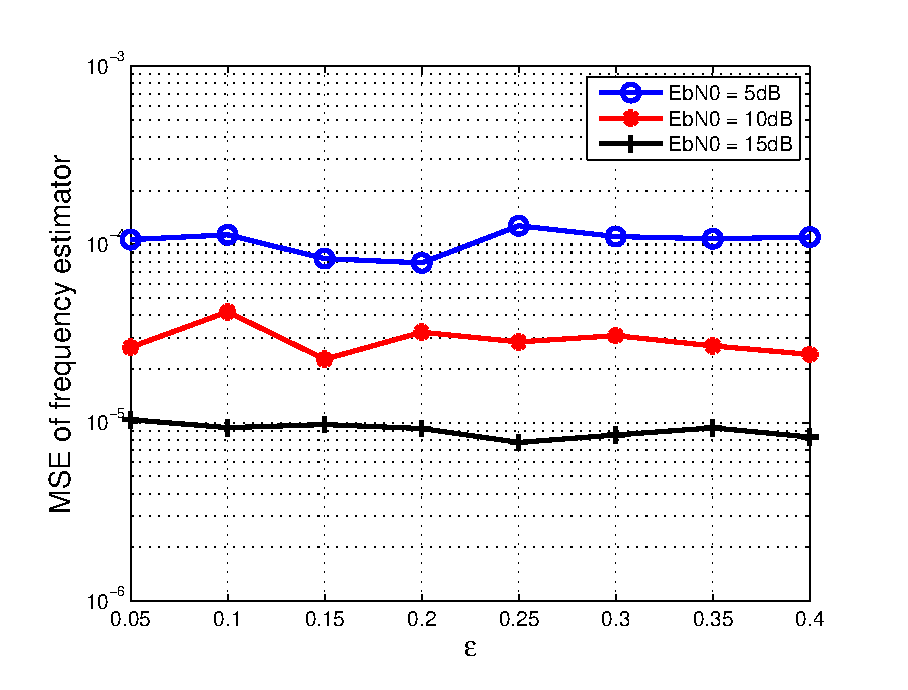
\includegraphics[width=0.4\textwidth]{plot_freqMSE_freqError_at_diffSNR.eps}
}
\subfigure[时间估计性能]
{
\label{plot_timeMSE_freqError_at_diffSNR}
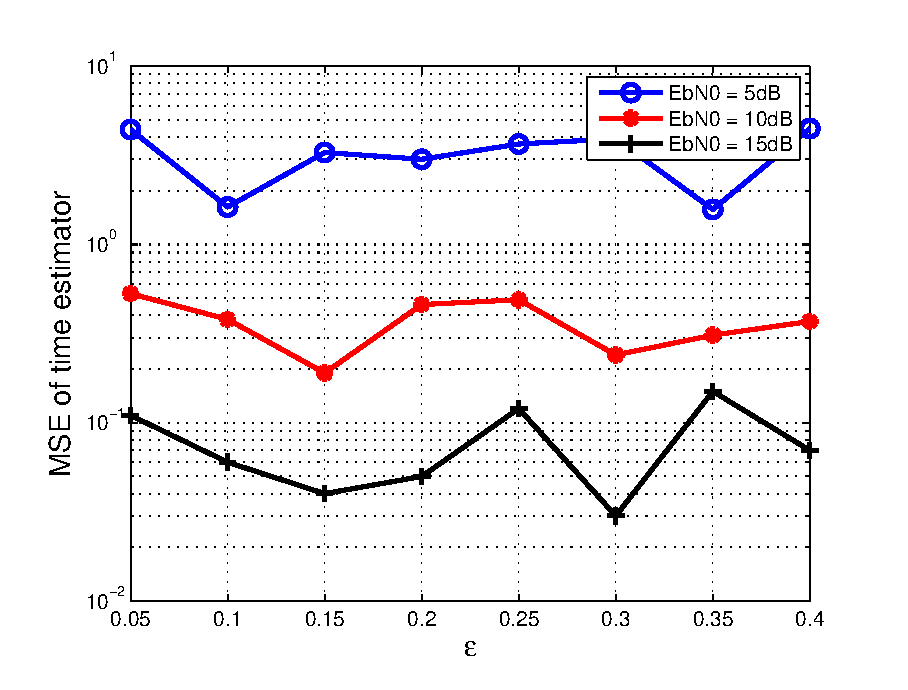
\includegraphics[width=0.4\textwidth]{plot_timeMSE_freqError_at_diffSNR.eps}
}
\caption{~ML~算法性能与频偏关系}\label{Performance_by_freqError}
\vspace{-1em}
\end{figure}
仿真条件为子载波数~2048~,循环前缀长度为~144。三条曲线信噪比分别取~5dB,10dB,15dB。归一化频偏值从~0.05~开始以~0.05~步进取到~0.4。首先显而易见的是信道条件越好,信噪比越大,估计的性能越好。还可以从图中看出无论频偏大小为多少,得到的频偏估计均方误差一定,即~ML~算法的频率偏移误差估计性能与频偏大小无关。

下面我们观察~ML~算法的估计性能都与哪些因素有关。图~\ref{Performance_by_alpha}~给出了不同阶数变换下算法的估计性能,仿真条件同样为子载波数~2048~,循环前缀长度为~144,归一化频率偏移为固定值~0.1。可以看出估计性能与混合载波通信系统的变换阶数无关。
\begin{figure}[htbp]
\centering
\subfigure[频率估计性能]
{
\label{plot_freqMSE_alpha_at_diffSNR}
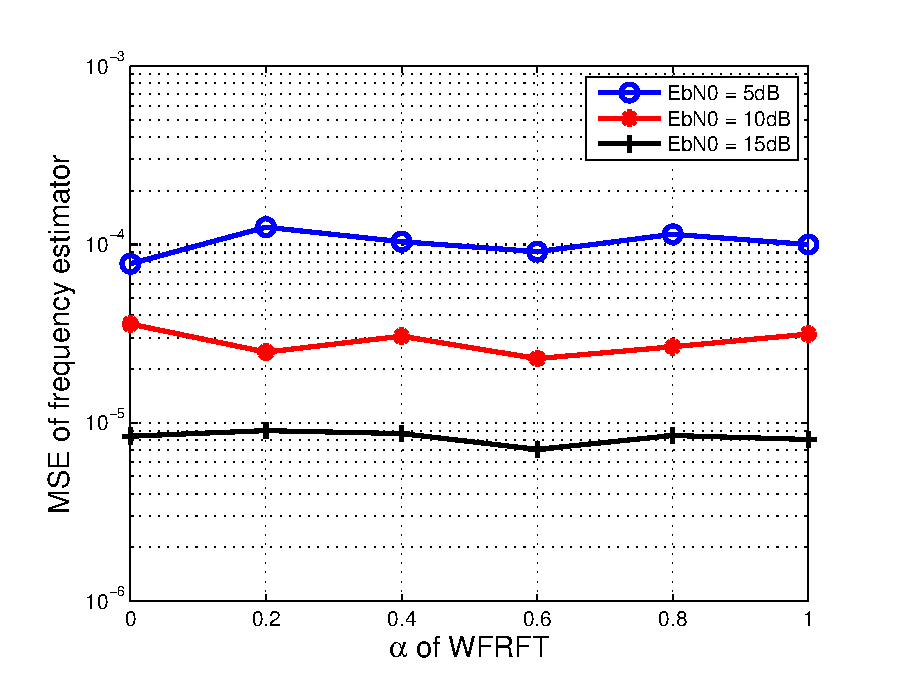
\includegraphics[width=0.4\textwidth]{plot_freqMSE_alpha_at_diffSNR.eps}
}
\subfigure[时间估计性能]
{
\label{plot_timeMSE_alpha_at_diffSNR}
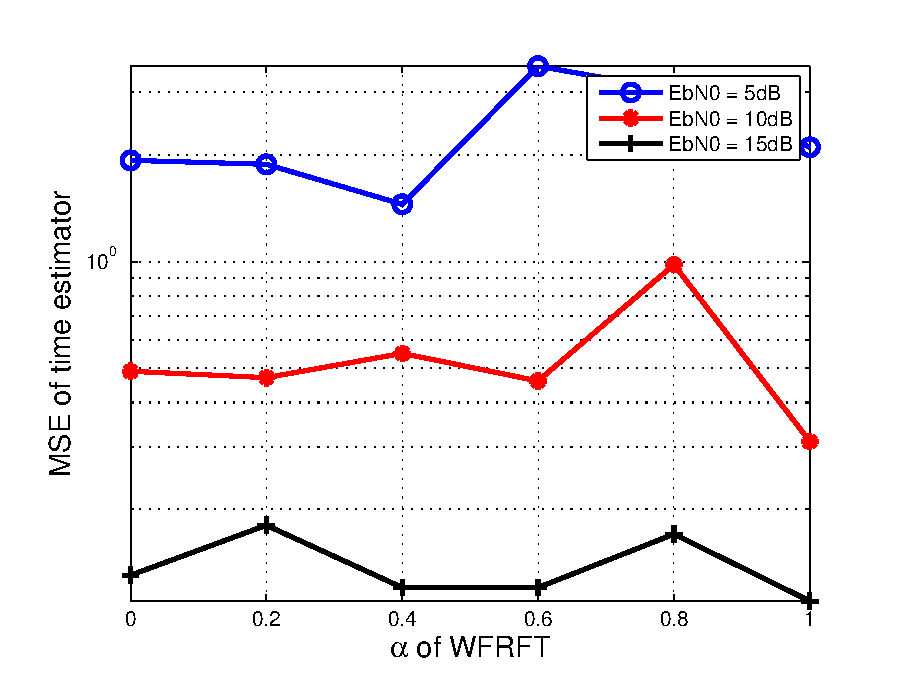
\includegraphics[width=0.4\textwidth]{plot_timeMSE_alpha_at_diffSNR.eps}
}
\caption{~ML~算法性能与变换阶数关系}\label{Performance_by_alpha}
\vspace{-1em}
\end{figure}

图~\ref{Performance_by_CP}~给出了不同循环前缀长度下定时估计和频偏估计的均方误差随循信噪比的变换关系。
\begin{figure}[htbp]
\centering
\subfigure[频率估计性能]
{
\label{plot_freqMSE_EbN0_at_diffCP}
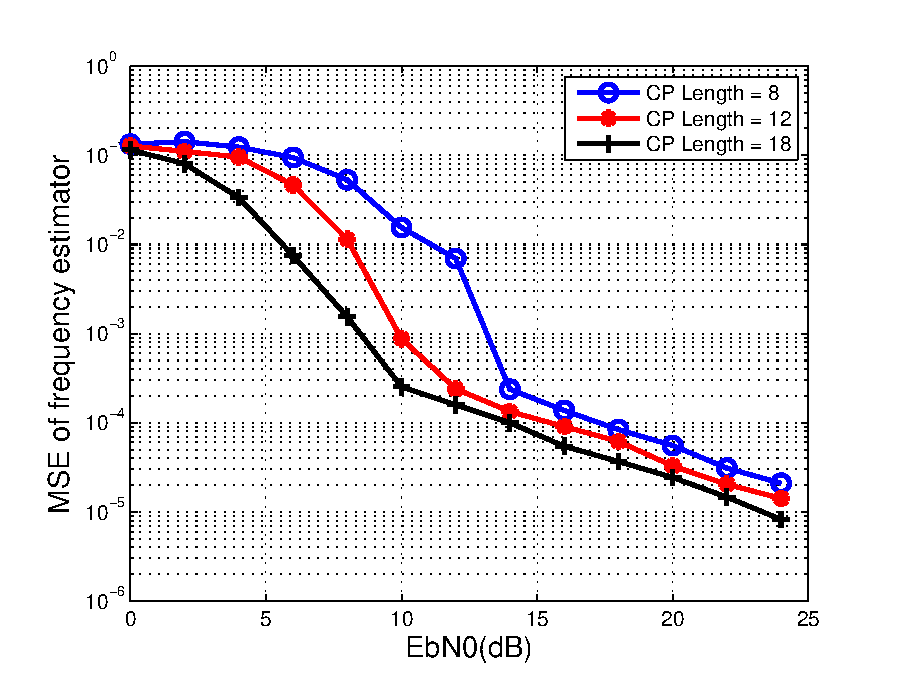
\includegraphics[width=0.4\textwidth]{plot_freqMSE_EbN0_at_diffCP.eps}
}
\subfigure[时间估计性能]
{
\label{plot_timeMSE_EbN0_at_diffCP}
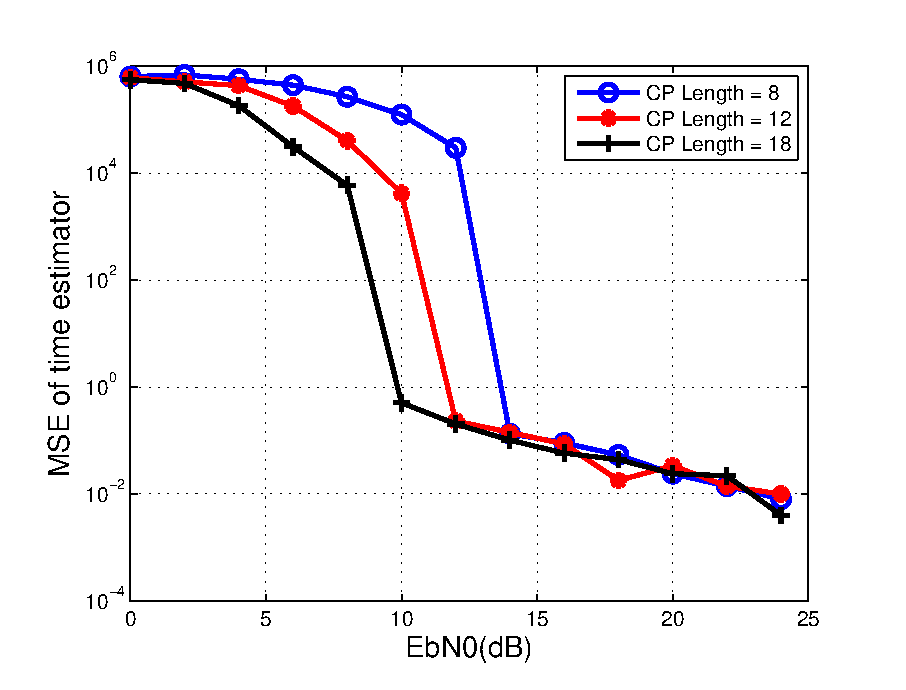
\includegraphics[width=0.4\textwidth]{plot_timeMSE_EbN0_at_diffCP.eps}
}
\caption{~ML~算法性能与循环前缀长度关系}\label{Performance_by_CP}
\vspace{-1em}
\end{figure}
仿真条件为子载波数~2048~,分别去循环长度为~8,12,18。归一化频偏设定为~0.25。可以看出,在同一信噪比条件下,频偏估计均方误差随着循环前缀的增加而下降,当超过一定门限(约12dB)时,均方误差随着信噪比的下降趋势会便缓慢,但是同定时估计性能相比下降的更为明显。在门限之前,循环前缀越长,同一信噪比下所对应的频率同步均方误差越小,而超过此特定门限之后,增加循环前缀所带来的性能优势仍然存在但变得不再明显。而定时估计性能同样存在一个门限(约12dB),在随信噪比的增加通过门限时不同长度循环前缀的定时估计均方误差迅速下降,趋于重合,说明超过门限之后不同循环前缀长度的定时同步性能已经基本相同。

从最大似然函数的表达式不难看出,每计算一个采样点的计算量较大,在实际实现过程中比较困难。为了解决这个问题,压缩同步算法的运算量,文献\cite{Muller1998On}提出了最大相关(MC)算法,它仅是~ML~算法的简化算法,只考虑了~CP~与数据部分的相关性,计算复杂度大大降低。
MC~算法的最大似然函数为:
\begin{equation}
\Lambda \left( {\theta ,\varepsilon } \right) = {\left| {\gamma \left( \theta  \right)} \right|^2} = {\left| {\sum\limits_{n = \theta }^{\theta  + L - 1} {r\left( n \right){r^*}\left( {n + N} \right)} } \right|^2}
\end{equation}

因而得到的联合估计为:
\begin{align}
&{{\hat \theta }_{MC}} = \arg \mathop {\max }\limits_\theta  \left\{ {{{\left| {\gamma \left( \theta  \right)} \right|}^2}} \right\} \\
&{{\hat \varepsilon }_{MC}} =  - \frac{1}{{2\pi }}\angle \gamma \left( {{{\hat \theta }_{MC}}} \right)
\end{align}

下面给出~MC~算法的运算框图~\ref{MC_kuangtu}~。
\begin{figure}[htbp]
\centering
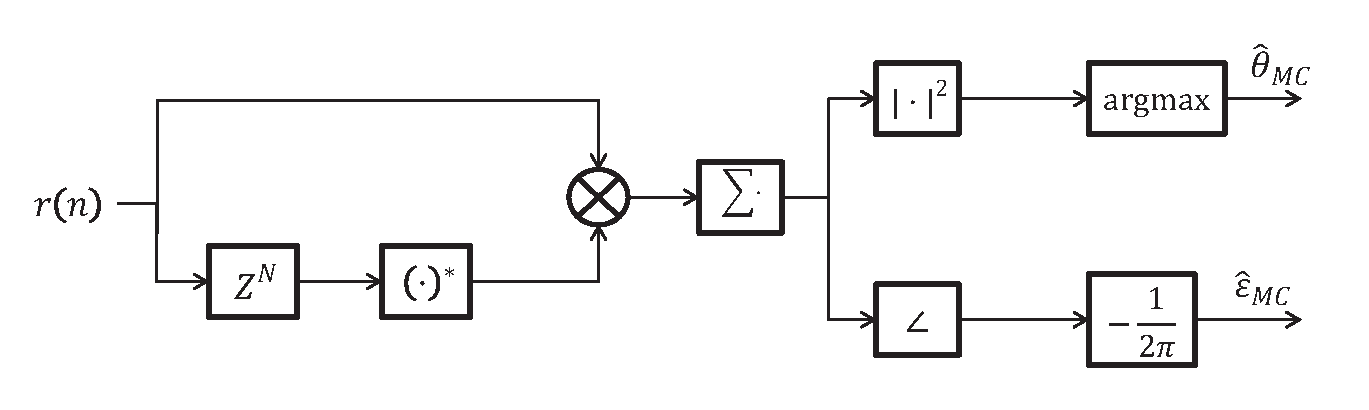
\includegraphics[width = 0.8\textwidth]{MC_kuangtu.eps}
\caption{~MC~算法框图}\vspace{-1em}\label{MC_kuangtu}
\end{figure}

可以看到运算复杂性大大降低,实际上从最大似然函数的表达式也能看出,ML~中的能量项被忽略,仅保留相关函数项,这对于频偏估计是没有影响的,但牺牲了定时估计的准确性。

综上所述,ML~算法应用在混合载波通信系统中,有着不占用额外频谱资源,同时计算量小的优点。但同时极易受到干扰,包括信道,滤波等等,都在一定程度上破坏CP前后一致性,可以通过联合多个符号~CP~同时,进行辅助同步,显著降低误差,虽然并未额外浪费频谱资源,但由于联合多个符号进行,会增加接收端信号处理延时。而在实际应用中,当存在多径干扰时,CP部分会与数据部分的相关性受到影响,此时的估计抖动较大,因为~ML~算法本事是以~AWGN~信道为前提而进行的,而无线通信中的信号基本都会受到严重的多径干扰,故如何有效抗多径干扰是此同步算法急需解决的问题。





